% ============================================================================
% E-DATA — Paper (versión revisada)
% Secciones revisadas contra el código del proyecto: 4 (Diseño del sistema:
% requerimientos, complejidad, diagrama general e historias de usuario),
% 5 (KPIs), 9 (Conclusiones) y Agradecimientos.
% Las demás secciones se transcribieron del PDF original SIN cambios.
% Para compilar en Overleaf: subir este archivo y "diagrama-general.png".
% ============================================================================
\documentclass[10pt,journal,compsoc]{IEEEtran}

\usepackage[utf8]{inputenc}
\usepackage[T1]{fontenc}
\usepackage[spanish,es-nodecimaldot,es-noshorthands,es-tabla]{babel} % es-tabla: "Tabla" en vez de "Cuadro"
\usepackage{amsmath,amssymb}
\usepackage{booktabs}
\usepackage{tabularx}
\usepackage{graphicx}
\usepackage{float}  % [H] deja una tabla exactamente donde se escribe
\usepackage{url}

\renewcommand{\IEEEkeywordsname}{Index Terms}

\begin{document}

\title{E-DATA: Plataforma Informativa de Monitoreo Energético Basada en Inteligencia Artificial Local y Estructuras de Datos Eficientes}

\author{Daniel~Felipe~Cárdenas~Romero, Jerónimo~Urrego~and~Andrés~Rubio
\IEEEcompsocitemizethanks{\IEEEcompsocthanksitem D. F. Cárdenas Romero y J. Urrego pertenecen al Programa de Ingeniería de Inteligencia Artificial, y A. Rubio al Programa de Ingeniería de Ciberseguridad, Escuela Colombiana de Ingeniería Julio Garavito, Bogotá, Colombia.\protect\\
E-mail: daniel.cardenas-r@mail.escuelaing.edu.co, jeronimourrego.88@gmail.com, andres.rubio@mail.escuelaing.edu.co}}

\IEEEtitleabstractindextext{%
\begin{abstract}
El consumo ineficiente de energía en los entornos residenciales genera sobrecostos significativos debido al ``consumo fantasma'' (dispositivos conectados en estado de reposo) y a las recientes penalizaciones regulatorias por exceder las metas de gasto promedio. Estas ineficiencias, a menudo imperceptibles para el usuario común, pueden incrementar la facturación eléctrica hasta en un 15\%. Para abordar esta problemática, en alineación con el Objetivo de Desarrollo Sostenible (ODS) 7 (Energía asequible y no contaminante), la presente investigación detalla la arquitectura teórica y el desarrollo de E-DATA, una plataforma de monitoreo energético impulsada por estructuras de datos avanzadas (Árboles N-arios y Colas de Prioridad Max-Heap) y modelos de inferencia de Inteligencia Artificial (IA). A diferencia de los Sistemas de Gestión de Energía en el Hogar (HEMS) convencionales, que dependen de infraestructuras de computación en la nube de alta latencia o intervenciones automatizadas de hardware intrusivas, este sistema despliega un análisis de datos delegado a una red neuronal de ejecución local (Gemma 4 E4B), operando mediante un servidor simulado en Python a través de FastAPI. La plataforma procesa historiales de consumo, ejecuta simulaciones financieras con una tarifa de referencia del mercado colombiano, en el contexto de la Resolución CREG 101-120 de 2026, y actúa como un analista consultivo. Al generar sugerencias personalizadas en lenguaje natural orientadas a la economía conductual, la solución empodera a los usuarios para mitigar el consumo vampiro, facilitando una reducción del consumo general de hasta un 15\% y contribuyendo a cumplir las metas de ahorro sin ceder el control domótico del hogar.
\end{abstract}

\begin{IEEEkeywords}
Inteligencia Artificial Local, Edge AI, Gemma 4 E4B, Monitoreo Energético, Árbol N-ario, Max-Heap, CREG 101-120, Economía Conductual.
\end{IEEEkeywords}}

\maketitle
\IEEEdisplaynontitleabstractindextext
\IEEEpeerreviewmaketitle

% ============================================================================
\section{Introducción}
% ============================================================================
\IEEEPARstart{E}{l} acceso continuo, seguro y eficiente a la energía eléctrica es un pilar indispensable para el desarrollo de la sociedad moderna. Sin embargo, la gestión inadecuada de este recurso en el sector residencial representa un desafío crítico tanto para la sostenibilidad ambiental global como para la estabilidad económica doméstica \cite{xue2025}. A nivel macroscópico, el consumo ineficiente en los hogares contribuye de manera desproporcionada a la huella de carbono, exacerbando los efectos del cambio climático. A nivel microeconómico, gran parte de este desperdicio energético proviene del denominado ``consumo fantasma'' o \emph{vampire draw}, generado por aparatos que, aun estando apagados o inactivos, permanecen conectados a la red eléctrica y consumen energía en estado de espera (\emph{standby}) \cite{dalln2016}. A pesar de los avances en la medición inteligente, la vasta mayoría de los usuarios residenciales carecen de herramientas granulares que les permitan visibilizar qué dispositivos específicos de su topología doméstica lideran este consumo pasivo.

En el contexto específico de Colombia, esta problemática de ineficiencia ha adquirido una urgencia regulatoria inminente. Ante fenómenos climáticos severos como El Niño, que amenazan drásticamente los niveles de los embalses hidroeléctricos (fuente principal de la matriz energética del país), el Gobierno Nacional a través de la Comisión de Regulación de Energía y Gas (CREG) emitió la Resolución 101-120 de 2026 \cite{creg2026}. Este marco regulatorio establece un programa transitorio, automático y de obligatorio cumplimiento que penaliza económicamente a los usuarios regulados cuyo consumo exceda el 110\% de su meta histórica de consumo (calculada mediante la mediana estadística de los últimos 12 meses) \cite{creg2026}. Las penalizaciones imponen recargos severos del 30\%, 50\% o 70\% sobre la tarifa base de energía (aproximadamente 875 COP/kWh), dependiendo del estrato socioeconómico o del sector (residencial, comercial o industrial) \cite{creg2026}. Simultáneamente, el mismo marco prevé incentivos económicos para aquellos usuarios que logren reducir su gasto por debajo del 90\% de dicha meta.

En respuesta a este complejo panorama hidro-climático y regulatorio, surge E-DATA, una solución arquitectónica de software de vanguardia. La propuesta central de este proyecto radica en sustituir las métricas incomprensibles de los medidores tradicionales, que usualmente reportan un volumen agregado en kilovatios-hora, por un programa de monitoreo inteligente que transforma la topología física de la vivienda en estructuras algorítmicas puras \cite{xue2025}. Integrando una Inteligencia Artificial local (el modelo Gemma 4 E4B, optimizado para operaciones en el borde) conectada a un entorno de backend asíncrono en Python, E-DATA funciona como un asesor energético automatizado. El sistema evalúa continuamente los requerimientos presupuestales del usuario, aísla el consumo en reposo mediante Colas de Prioridad, y genera recomendaciones no intrusivas en lenguaje natural. De esta forma, la plataforma promueve el ahorro voluntario, protegiendo a los hogares de las agresivas sanciones regulatorias, maximizando la privacidad de los datos al mantener la inferencia algorítmica de manera local, y apoyando indirectamente la estabilización de la red eléctrica nacional.

% ============================================================================
\section{Justificación}
% ============================================================================
El diseño y desarrollo de E-DATA se fundamenta en tres ejes críticos que justifican su viabilidad técnica, su impacto financiero y su pertinencia frente a las soluciones de automatización tradicionales: el impacto financiero del consumo en espera, la necesidad de una arquitectura de baja latencia con alta soberanía de datos, y la integración de la economía conductual en la interacción humano-máquina.

\subsection{El Eje Financiero y Regulatorio}
El consumo fantasma no es una métrica marginal; estimaciones del Departamento de Energía y laboratorios de investigación indican que el \emph{vampire draw} puede representar entre el 5\% y el 10\% del consumo eléctrico total en un hogar promedio, y en ecosistemas altamente tecnificados, puede superar el 15\% \cite{dalln2016}. Considerando la tarifa vigente en el mercado eléctrico colombiano (promediando 875.04 COP/kWh), un hogar que desperdicia pasivamente tan solo 40 Watts constantes incurre en un consumo adicional de 28.8 kWh al mes, lo que se traduce en un gasto innecesario de aproximadamente \$300,000 COP anuales \cite{creg2026}.

Bajo las estrictas directrices de la Resolución CREG 101-120 de 2026, el impacto de este desperdicio se magnifica exponencialmente. Si el consumo fantasma empuja a un usuario residencial (e.g., estrato 4) por encima del margen de tolerancia del 110\% de su meta de consumo, el sobrecosto aplicado no es estándar, sino que acarrea una penalización del 50\% extra sobre la tarifa \cite{creg2026}. Por tanto, la identificación milimétrica de las cargas vampiro es una necesidad financiera. E-DATA monetiza la visualización de los datos (mostrando el gasto y el ahorro potencial directamente en Pesos Colombianos), atacando de inmediato este segmento del consumo y brindando una herramienta para mantener al hogar dentro de la ``banda neutra'' tarifaria.

\subsection{El Eje Arquitectónico y de Privacidad (Edge AI)}
Históricamente, las aplicaciones de Monitoreo de Carga No Intrusiva (NILM) o los Sistemas de Gestión de Energía en el Hogar (HEMS) requieren el envío constante de datos de telemetría de alta frecuencia a servidores centralizados en la nube para su procesamiento algorítmico \cite{xue2025}. Esto introduce dos vectores de fallo masivos: vulnerabilidades de privacidad (la exposición de patrones de vida del usuario a terceros) y latencias dependientes de la red.

E-DATA plantea un paradigma de infraestructura diametralmente opuesto al utilizar estructuras de datos nativas (Árboles N-arios y Colas de Prioridad) para pre-filtrar y ordenar matemáticamente los electrodomésticos antes de invocar a la IA. Al integrar Gemma 4 E4B, un modelo de lenguaje de tamaño reducido diseñado específicamente para dispositivos periféricos (\emph{Edge AI}) capaz de inferir eficientemente en CPUs comerciales y memoria RAM estándar, el sistema garantiza una soberanía de datos absoluta. Toda la inferencia y el empaquetamiento de las recomendaciones ocurre \emph{on-premise} sin depender de APIs de terceros (e.g., OpenAI o Anthropic), eliminando costos recurrentes de servidor y riesgos de interceptación de datos de la red doméstica.

\subsection{El Eje de la Economía Conductual}
Los optimizadores domóticos tradicionales se basan en relés de estado sólido que interrumpen el suministro de energía de forma abrupta a través de la intervención directa de la máquina. Este enfoque determinista genera una alta fricción con los usuarios, quienes a menudo perciben una pérdida de control sobre su propio hogar, derivando en la desactivación del sistema \cite{xue2025}.

E-DATA adopta un enfoque basado en la persuasión y la psicología cognitiva. La aversión a la pérdida se estimula mostrando el impacto monetario proyectado del consumo fantasma, en un contexto en el que la CREG ya penaliza los excesos \cite{xue2025}. En paralelo, la IA actúa como un mediador diplomático, dialogando de manera amigable para sugerir la desconexión manual de equipos no críticos. El humano retiene la agencia total de las decisiones, lo que fomenta una educación energética sostenible y cambios de hábitos a largo plazo.

% ============================================================================
\section{Estado del Arte}
% ============================================================================
La concepción arquitectónica de E-DATA se sitúa en la intersección de varias disciplinas de la ingeniería eléctrica, la ciencia de datos, y la inteligencia artificial distribuida. A continuación, se presenta un análisis exhaustivo del estado del arte, dividido en investigaciones internacionales y avances específicos del contexto nacional colombiano.

\subsection{Investigaciones Internacionales}
El desarrollo del marco lógico de E-DATA se fundamenta en recientes avances científicos globales que abordan el monitoreo eléctrico, la estructuración de datos y la inferencia de lenguaje en el borde:
\begin{enumerate}
\item \textbf{Monitoreo NILM \emph{Training-Free} mediante LLMs:} Tradicionalmente, la desagregación de la señal eléctrica principal de una vivienda en dispositivos individuales (NILM) requería algoritmos matemáticos complejos. Investigaciones recientes de Xue et al. (2025) demuestran que los LLMs pueden realizar inferencias NILM sin entrenamiento previo mediante \emph{prompt engineering} avanzado \cite{xue2025}. E-DATA aplica este concepto al empaquetar datos pre-procesados y delegar el reconocimiento de patrones a la red neuronal.
\item \textbf{Inferencia de Modelos en el Borde (Edge-LLM) y Partición de Caché:} Estudios sobre la arquitectura \emph{Edge-LLM} (Habibi et al., 2025; Cui et al., 2026) discuten mecanismos de asignación de capas y partición de la caché \emph{Key-Value} (KV) bajo limitaciones de RAM \cite{habibi2025,cui2026}. Gemma 4 E4B aprovecha el framework LiteRT-LM para procesar contextos a más de 6 t/s en procesadores comerciales \cite{hf2026}.
\item \textbf{Optimización Estructural y Baja Latencia en Entornos IoT:} Revisiones comparativas lideradas por Ala'anzy et al. (2025) concluyen que los árboles de búsqueda estructurados y las colas de prioridad minimizan la latencia frente a matrices planas \cite{alaanzy2025}. E-DATA implementa Árboles N-arios y Max-Heap para reducir la complejidad computacional.
\item \textbf{Modelado y Caracterización Matemática del Consumo Fantasma:} Dispositivos heredados como decodificadores sostienen extracciones pasivas superiores a 10W continuos \cite{dalln2016}. E-DATA utiliza estas clasificaciones para construir perfiles paramétricos precisos.
\item \textbf{Diseño de Interfaz y Retroalimentación Conductual:} Dalln \& Kraemer (2016) establecieron que traducir métricas de ingeniería a representaciones monetarias directas logra reducciones del gasto del 10\% al 15\% mediante persuasión pasiva \cite{dalln2016}.
\end{enumerate}

\subsection{Investigaciones y Contexto Nacional (Colombia)}
\begin{enumerate}
\item \textbf{Regulación Tarifaria y Penalizaciones (Resolución CREG 101-120 de 2026):} La norma impone recargos del 30\% al 70\% sobre consumos que excedan el 110\% de la meta individual \cite{creg2026}. Esta norma es el contexto que motiva a E-DATA: su motor estima el consumo, el costo y el ahorro del hogar, aunque no calcula las metas ni los recargos que ella define.
\item \textbf{Sistemas de Gestión de Energía (HEMS):} Araque-Gallardo (2023) se enfoca en optimización meta-heurística para almacenamiento físico pesado \cite{araque2023}. E-DATA propone una alternativa en software ligero para atacar la base conductual.
\item \textbf{Prototipos de Monitoreo IoT Residencial:} Investigaciones de la Universidad Uniagustiniana (2022) desarrollaron prototipos con sensores ACS712 y ESP32 \cite{uniagustiniana2022}, pero adolecen de capas analíticas autónomas. E-DATA provee el ``cerebro'' algorítmico local.
\item \textbf{Eficiencia Energética en Edificaciones:} Estudios de la UAC (2025) identificaron la dependencia de internet como una vulnerabilidad en monitoreo IoT \cite{uac2025}. La arquitectura \emph{Edge} de E-DATA resuelve esta limitación.
\item \textbf{Infraestructura de Medición Avanzada (AMI):} Téllez-Gutiérrez et al. (2018) detallan la lentitud en la masificación de medidores inteligentes en Colombia \cite{tellez2018}. E-DATA representa una alternativa de software inmediata y escalable.
\end{enumerate}

% ============================================================================
\section{Diseño del Sistema}
% ============================================================================
% Las tres tablas de requisitos van juntas en una página propia (como en la versión original):
% así no quedan sueltas en medio de otras secciones.
\begin{table*}[p]
\centering
\footnotesize
\renewcommand{\arraystretch}{0.97}
\caption{Requerimientos Funcionales de Modelado y Captura (REQF 01--10)}
\label{tab:reqf1}
\begin{tabularx}{\textwidth}{@{}l l X@{}}
\toprule
\textbf{ID} & \textbf{Requerimiento} & \textbf{Criterio de Validación} \\
\midrule
\textbf{REQF-01} & Modelado de habitaciones & Crea y elimina habitaciones con nombre propio; rechaza un nombre repetido y una séptima habitación. \\
\textbf{REQF-02} & Catálogo de dispositivos & Muestra los 86 equipos con foto, marcas y potencia activa y en reposo (W); sin foto, muestra un ícono. \\
\textbf{REQF-03} & Búsqueda y filtro & La búsqueda por nombre o marca ignora tildes y mayúsculas (``bano'' encuentra ``Baño'') y se combina con el filtro por zona. \\
\textbf{REQF-04} & Sincronización de zona & Al elegir un dispositivo o una zona, el destino pasa a la habitación que coincide (nevera $\rightarrow$ Cocina). \\
\textbf{REQF-05} & Lógica condicional por tipo & \emph{Variable}: pide minutos de uso (propone un valor típico) y si queda conectado. \emph{Cíclico}: 30\% del día (7,2 h). \emph{Continuo}: 24 h. En los dos últimos se ocultan los campos de uso. \\
\textbf{REQF-06} & Inventario por habitación & El panel ``Mis dispositivos'' lista lo instalado por habitación y permite eliminarlo; cualquier cambio invalida la simulación anterior. \\
\textbf{REQF-07} & Representación isométrica & La casa se dibuja con suelo, paredes, muebles y dispositivos (los 86 con dibujo propio; si no queda sitio libre, un marcador con ícono); al pasar el mouse se ve la ficha del equipo. \\
\textbf{REQF-08} & Navegación en la vivienda & El avatar se mueve con teclado o clic siguiendo el camino más corto (BFS) sin atravesar paredes; la vista admite zoom de 0,7$\times$ a 4$\times$ y arrastre. \\
\textbf{REQF-09} & Validación de la petición & Una petición con tipos erróneos o campos faltantes recibe HTTP 422 sin ejecutar el cálculo. \\
\textbf{REQF-10} & Estructura jerárquica & La vivienda se recibe como árbol N-ario de tres niveles (casa $\rightarrow$ habitaciones $\rightarrow$ dispositivos) y se recorre completa una sola vez. \\
\bottomrule
\end{tabularx}
\vspace{0.9em}
\caption{Requerimientos Funcionales de Cálculo, Resultados e IA (REQF 11--20)}
\label{tab:reqf2}
\begin{tabularx}{\textwidth}{@{}l l X@{}}
\toprule
\textbf{ID} & \textbf{Requerimiento} & \textbf{Criterio de Validación} \\
\midrule
\textbf{REQF-11} & Consumo activo & Cada dispositivo aporta $P_{activo}\cdot t_{uso}/1000$ kWh al consumo del día. \\
\textbf{REQF-12} & Consumo en reposo & Solo si el equipo quedó conectado se suma $P_{standby}\cdot(24-t_{uso})/1000$ kWh; un equipo desconectado aporta 0. \\
\textbf{REQF-13} & Costo diario y mensual & Costo del día = kWh $\times$ tarifa (875,04 COP/kWh por defecto); costo del mes = costo del día $\times$ 30. \\
\textbf{REQF-14} & Ranking de vampiros & Solo entran equipos desconectables, conectados y con $P_{standby}>0$; la lista sale ordenada de mayor a menor potencia en reposo. \\
\textbf{REQF-15} & Ahorro potencial & El ahorro al mes es exactamente el consumo en reposo de los vampiros $\times$ 30 días $\times$ tarifa; el anual es el mensual $\times$ 12. \\
\textbf{REQF-16} & Prompt unificado & El texto para la IA contiene solo cifras ya calculadas: si se respetó el presupuesto diario, gasto del día, proyección mensual, vampiros y ahorro. \\
\textbf{REQF-17} & Consulta a la IA local & \texttt{POST /api/ia} envía el \emph{prompt} a \texttt{localhost:1234/v1/chat/completions} con el rol ``AI Analyst de E-DATA'' y devuelve un párrafo. \\
\textbf{REQF-18} & Simulación visual del día & Un día de 24 h transcurre en 2 minutos con reloj de sol y luna, ciclo día/noche y contadores de kWh y COP que crecen hasta el valor calculado. \\
\textbf{REQF-19} & Panel de resultados & Al terminar el día simulado aparece el panel, sin esperar a la IA: ahorro al mes y al año, consumo y costo del día, costo del mes y ranking numerado con barras. \\
\textbf{REQF-20} & Estados del análisis & El botón principal pasa por ``Simular día'' $\rightarrow$ ``Calculando…'' $\rightarrow$ ``Ver análisis''; en el último estado abre el chat con la respuesta de la IA. \\
\bottomrule
\end{tabularx}
\vspace{0.9em}
\caption{Requerimientos No Funcionales del Sistema (REQNF 01--14)}
\label{tab:reqnf}
\begin{tabularx}{\textwidth}{@{}l l X@{}}
\toprule
\textbf{ID} & \textbf{Criterio} & \textbf{Especificación Técnica} \\
\midrule
\textbf{REQNF-01} & Complejidad acotada & La simulación completa cuesta $O(n + v\log v)$, con $v \le n$; cada inserción o extracción del heap es $O(\log v)$. \\
\textbf{REQNF-02} & Recorrido lineal & Consumo, costo y ahorro se calculan en un único recorrido $O(n)$ sin ciclos anidados entre dispositivos. \\
\textbf{REQNF-03} & Validación tipada & Esquemas de Pydantic (\texttt{Dispositivo}, \texttt{Habitacion}, \texttt{SimulacionRequest}) rechazan datos mal formados. \\
\textbf{REQNF-04} & Desacople de capas & Frontend, backend e IA son procesos independientes; el panel de resultados se muestra aunque la IA no responda. \\
\textbf{REQNF-05} & Control de generación & Temperatura $T = 0{,}6$, límite de 1500 tokens y respuesta en un solo párrafo. \\
\textbf{REQNF-06} & Privacidad local & Los datos de la vivienda solo viajan entre el navegador, \texttt{127.0.0.1:8000} y \texttt{localhost:1234}; ninguna API externa recibe información del usuario. \\
\textbf{REQNF-07} & Cifras deterministas & Los kWh y los pesos se calculan en Python y se inyectan en el \emph{prompt}; la IA no hace cálculos y el panel usa las cifras del backend. \\
\textbf{REQNF-08} & Manejo de excepciones & Si LM Studio falla, \texttt{/api/ia} responde un JSON con el error; si el backend no responde, la interfaz avisa y vuelve al estado inicial. \\
\textbf{REQNF-09} & Interfaz liviana & Estructura de la página lista (\emph{DOMContentLoaded}) en menos de 100 ms al servirse localmente. \\
\textbf{REQNF-10} & Tecnología simple & Frontend sin frameworks ni compilación; backend con FastAPI, Pydantic y el cliente de OpenAI como únicas bibliotecas. \\
\textbf{REQNF-11} & Formato monetario & Pesos con punto de miles (\$1.296) y kWh con coma decimal (1,48 kWh), según la convención es-CO. \\
\textbf{REQNF-12} & Retroalimentación visual & Modo oscuro verde (\#050d0a, esmeralda \#1c9a68, musgo \#86d36c), ámbar \#e9ad52 para vampiros y estados \emph{hover}/\emph{focus} visibles. \\
\textbf{REQNF-13} & Coherencia de resultados & Si la casa cambia o se lanza otra simulación, se descartan los resultados anteriores. \\
\textbf{REQNF-14} & Alineación conductual & La IA sugiere con tono amigable y la aplicación nunca desconecta equipos: decide el usuario. \\
\bottomrule
\end{tabularx}
\end{table*}

La arquitectura de E-DATA se compone de tres capas que se ejecutan como procesos independientes en el mismo equipo del usuario y se comunican por HTTP local:

\begin{itemize}
\item \textbf{Interfaz gráfica (Frontend):} HTML, CSS y JavaScript sin frameworks ni paso de compilación. Permite modelar la vivienda (hasta 6 habitaciones), elegir dispositivos de un catálogo de 86 equipos con su potencia activa y en reposo, y ver la casa en una vista isométrica con un avatar que se desplaza por ella. También anima la simulación de un día y presenta los resultados.
\item \textbf{Motor de cálculo (Backend):} API en Python con FastAPI y validación de datos con Pydantic. Expone \texttt{POST /api/simular}, que calcula el consumo, el costo, el ahorro potencial y el ranking de dispositivos vampiro, y \texttt{POST /api/ia}, que reenvía al modelo de lenguaje el \emph{prompt} construido con esas cifras.
\item \textbf{Motor de inferencia (IA local):} servidor LM Studio en \texttt{localhost:1234} con el modelo cuantizado Gemma 4 E4B, consultado mediante su API compatible con OpenAI.
\end{itemize}

\subsection{Requerimientos Funcionales (REQF)}
Las Tablas~\ref{tab:reqf1} y \ref{tab:reqf2} resumen los 20 requerimientos funcionales, agrupados según el recorrido del usuario. Los diez primeros cubren el modelado de la vivienda: crear habitaciones, elegir dispositivos del catálogo, verlos en la casa isométrica y enviarlos al backend con una estructura válida. Los diez siguientes cubren lo que ocurre al simular: el cálculo del consumo, el costo y el ahorro, el ranking de vampiros, la animación del día, el panel de resultados y la consulta a la IA local.

Cada criterio de validación describe una acción concreta y su resultado esperado, de modo que puede comprobarse directamente sobre el sistema construido: en la interfaz, enviando peticiones a \texttt{/api/simular} o, en el caso de la IA, con LM Studio en ejecución.

\subsection{Requerimientos No Funcionales (REQNF)}
La Tabla~\ref{tab:reqnf} especifica las restricciones de calidad del sistema. Se agrupan en cuatro frentes: eficiencia (complejidad, recorrido lineal y carga de la interfaz), confiabilidad (validación tipada, cifras deterministas, manejo de errores y coherencia de resultados), privacidad y desacople entre capas, y experiencia del usuario (formato monetario, retroalimentación visual y alineación conductual). Los valores medidos se obtuvieron en el equipo de desarrollo y se detallan en la sección~\ref{sec:complejidad} y en los KPIs técnicos.

\subsection{Diagrama General}
La Fig.~\ref{fig:diagrama} muestra las tres capas y el flujo de una simulación. El usuario arma su casa en el frontend (1); al pulsar ``Simular día'' el navegador envía la vivienda en JSON a \texttt{/api/simular} (2), que la valida, la recorre, ordena los vampiros en el heap y devuelve kWh, costos, ahorro, ranking y el \emph{prompt} (3). Con esas cifras arrancan la animación del día y, al terminar, el panel de resultados. En paralelo, el frontend envía el \emph{prompt} a \texttt{/api/ia} (4), que consulta a Gemma 4 en LM Studio (5) y devuelve su recomendación (6) al chat. Finalmente, el usuario decide qué desconectar (7).

\begin{figure*}[!t]
\centering
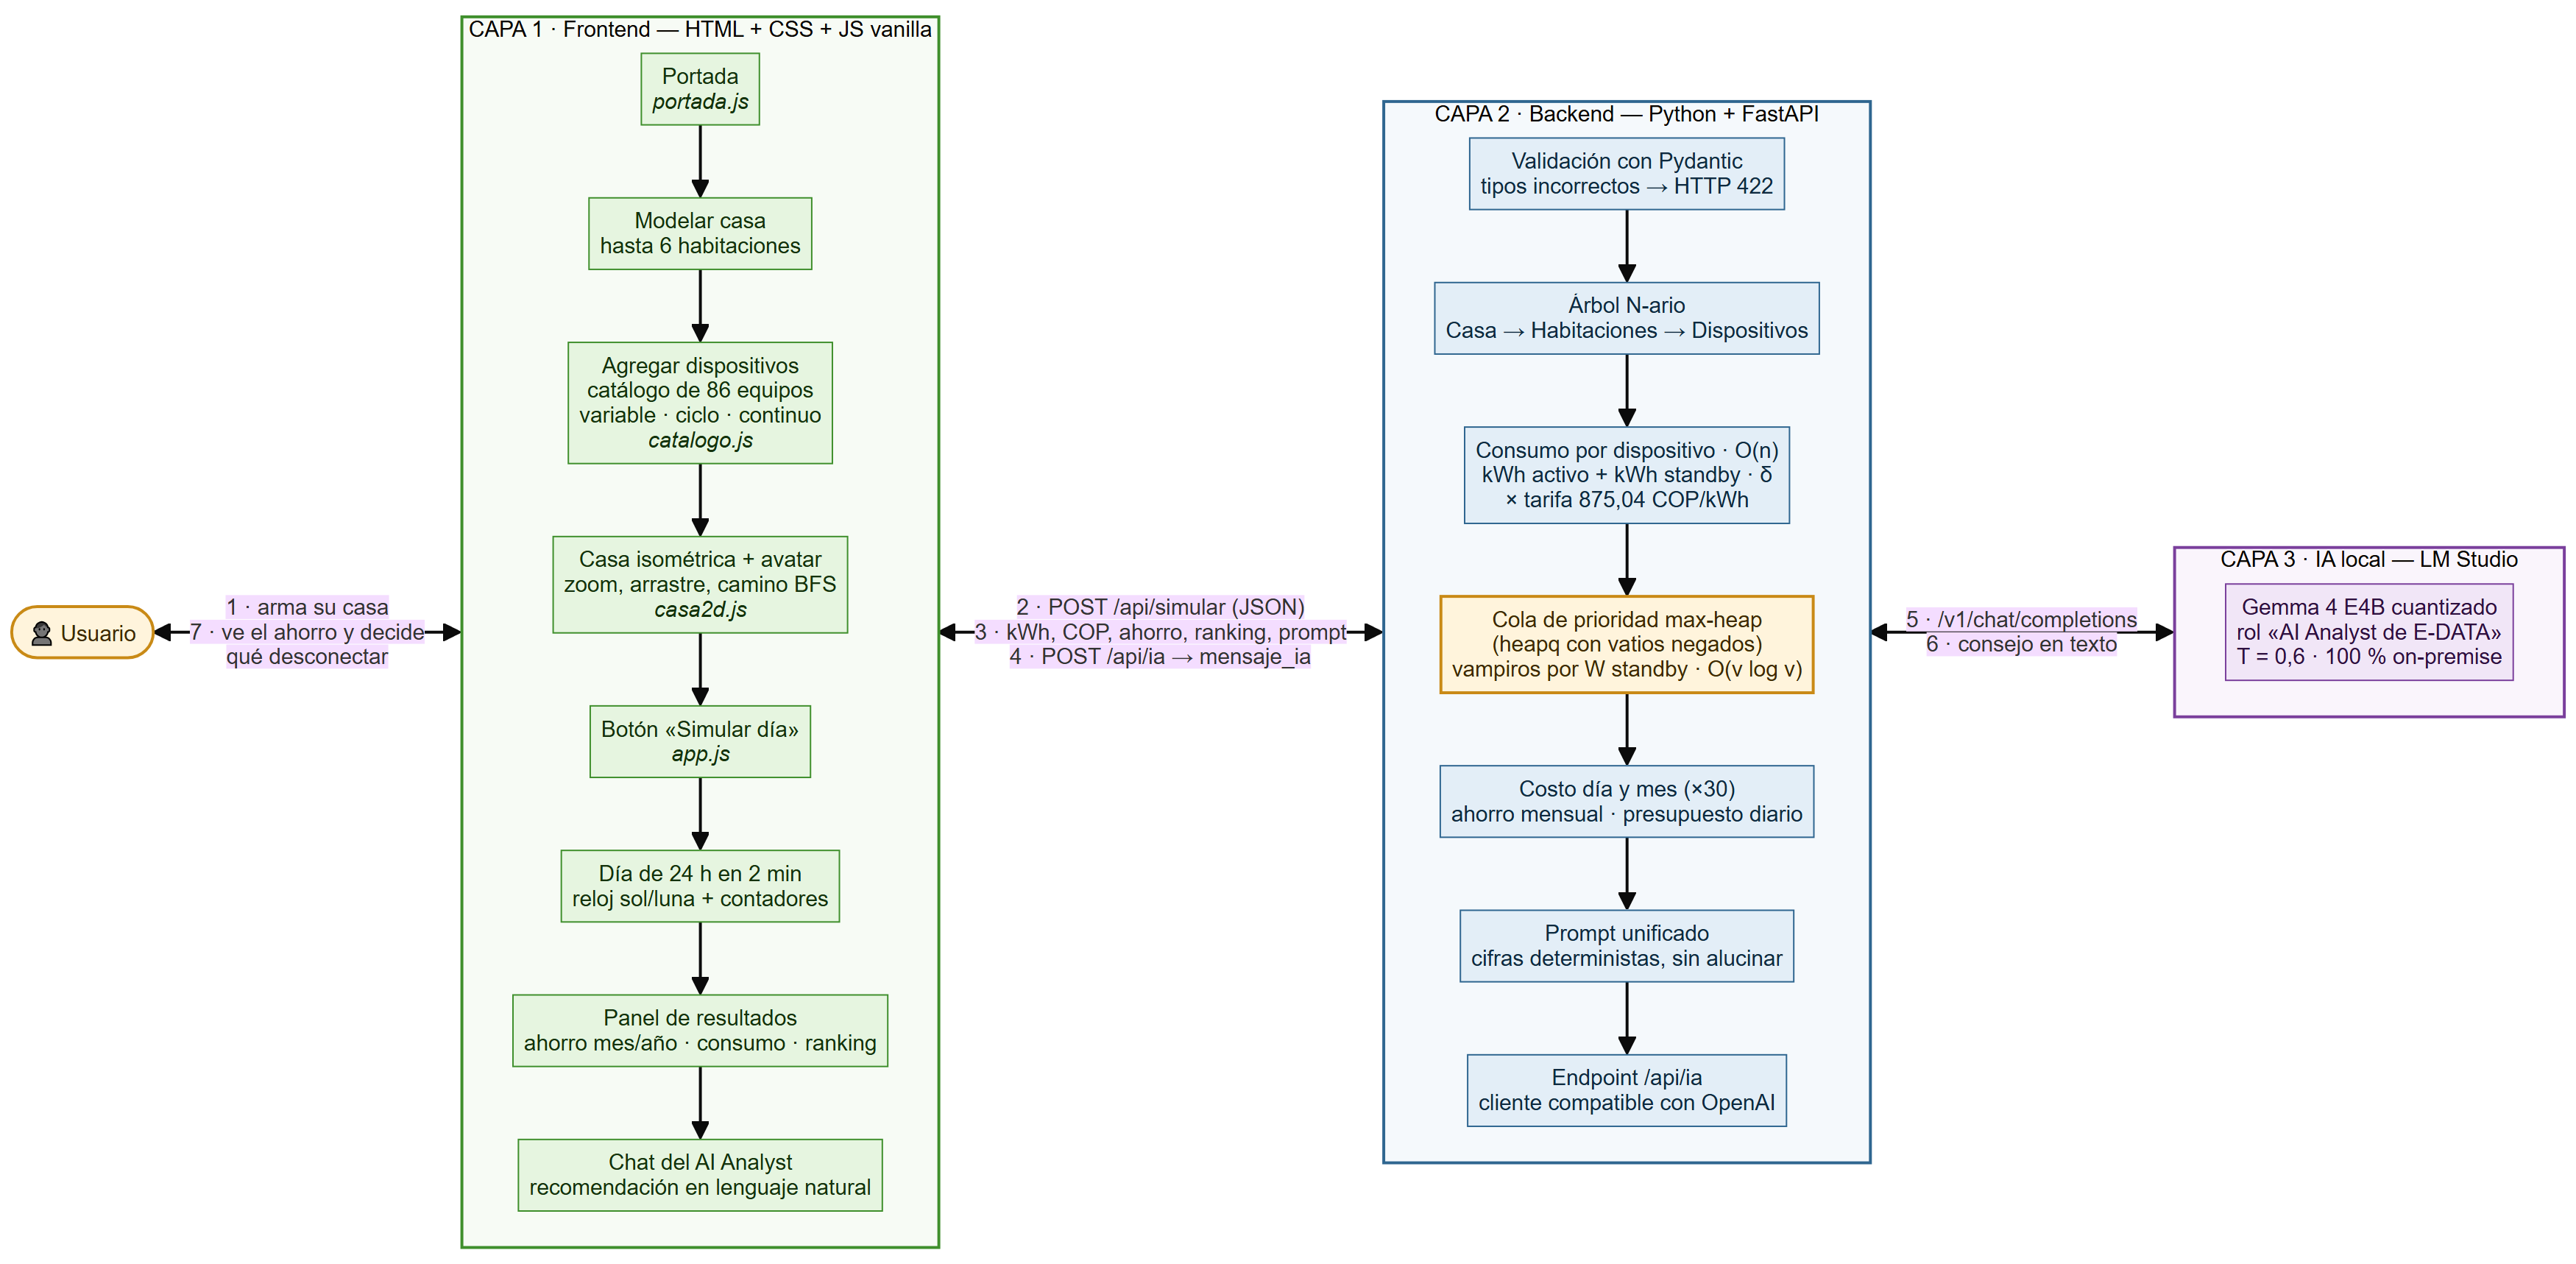
\includegraphics[width=\textwidth]{diagrama-general.png}
\caption{Diagrama general de E-DATA: capas, componentes y flujo de una simulación.}
\label{fig:diagrama}
\end{figure*}

% Salto de página: la página de tablas de requisitos (y luego la figura) sale aquí,
% entre dos subsecciones, para que la de complejidad empiece y termine sin cortes.
\newpage

\subsection{Modelado Matemático y Complejidad Asintótica (Big-O)}
\label{sec:complejidad}
Para una vivienda con $n$ dispositivos, modelados como las hojas del árbol N-ario, el costo diario en pesos colombianos ($C_{COP}$) se calcula como:
\begin{equation}
\begin{split}
C_{COP} = \text{Tarifa}\cdot\sum_{i=1}^{n}\Bigg[&\frac{P_{activo,i}\,t_{uso,i}}{1000}\\
&+ \frac{P_{standby,i}\,(24-t_{uso,i})\,\delta_i}{1000}\Bigg]
\end{split}
\label{eq:costo}
\end{equation}
donde Tarifa $=875{,}04$ COP/kWh (valor por defecto del sistema), las potencias $P$ están en vatios y $t_{uso,i}$ en horas: la que indica el usuario para equipos de uso variable, 7,2 h para los cíclicos y 24 h para los continuos. El parámetro conductual $\delta_i \in \{0,1\}$ vale 1 si el usuario dejó el equipo conectado y 0 si lo desconecta.

Sea $V$ el conjunto de vampiros: equipos con $\delta_i = 1$, desconectables y con $P_{standby,i} > 0$. El ahorro mensual potencial es exactamente el término de reposo de esos equipos:
\begin{equation}
A_{mes} = 30\cdot\text{Tarifa}\cdot\sum_{i\in V}\frac{P_{standby,i}\,(24-t_{uso,i})}{1000}
\label{eq:ahorro}
\end{equation}
y el ahorro anual es $A_{a\tilde{n}o} = 12\,A_{mes}$.

\textbf{Cola de prioridad.} Los vampiros se ordenan con un \emph{max-heap}: un árbol binario completo, guardado en un arreglo, donde cada padre es mayor o igual que sus hijos, de modo que la mayor fuga queda siempre en la cima. Python solo ofrece un \emph{min-heap} (\texttt{heapq}), así que se inserta la potencia con signo negativo ($-P_{standby}$): el menor de los negativos corresponde al mayor de los positivos.

\textbf{Complejidad.} Con $v = |V| \le n$:
\begin{itemize}
\item Recorrido del árbol y suma de consumos: $O(n)$.
\item $v$ inserciones en el heap, cada una $O(\log v)$: $O(v\log v)$.
\item $v$ extracciones de la cima para obtener el ranking ordenado: $O(v\log v)$.
\item Construcción del \emph{prompt}: $O(v)$.
\end{itemize}
El total es $O(n + v\log v)$, que en el peor caso ($v = n$) es $O(n\log n)$, con memoria adicional $O(v)$. En la interfaz, el filtrado del catálogo es $O(m)$ con $m = 86$, y la búsqueda de camino del avatar es un BFS sobre a lo sumo 96 celdas (6 habitaciones de $4\times4$).

\textbf{Verificación empírica.} Se midió la función de simulación con casas sintéticas de 10 habitaciones (promedio de 5 ejecuciones, sin servidor HTTP). La Tabla~\ref{tab:escalado} muestra que al multiplicar $n$ por 10 el tiempo crece cerca de 10 veces, como se espera de $O(n\log n)$ con un $\log$ pequeño.

\begin{table}[H]
\caption{Tiempo de la simulación según el número de dispositivos}
\label{tab:escalado}
\centering
\begin{tabular}{@{}rr@{}}
\toprule
\textbf{Dispositivos ($n$)} & \textbf{Tiempo (ms)} \\
\midrule
10 & 0,05 \\
100 & 0,32 \\
1.000 & 3,25 \\
10.000 & 37,9 \\
100.000 & 559,9 \\
\bottomrule
\end{tabular}
\end{table}

\subsection{Historias de Usuario}
Las siguientes historias describen lo que el sistema le permite hacer al usuario. Cada criterio de aceptación sigue el formato \emph{Dado / Cuando / Entonces} y puede comprobarse en la aplicación.

\textbf{HU-01. Modelar mi vivienda.} Como usuario, quiero crear las habitaciones de mi casa con sus propios nombres para ubicar cada dispositivo donde realmente está.
\begin{itemize}
\item Dado que escribo un nombre nuevo, cuando pulso agregar, entonces la habitación aparece en la lista, en el selector de destino y en la casa isométrica.
\item Dado que ya tengo 6 habitaciones o escribo un nombre repetido, cuando intento agregar otra, entonces el sistema la rechaza con un mensaje que explica por qué.
\item Dado que elimino una habitación, cuando la casa se vuelve a dibujar, entonces desaparecen sus dispositivos y la simulación anterior deja de mostrarse.
\end{itemize}

\textbf{HU-02. Agregar mis dispositivos.} Como usuario, quiero elegir mis aparatos de un catálogo con foto y consumo para no tener que conocer sus vatios.
\begin{itemize}
\item Dado que escribo ``bano'' en el buscador, cuando se filtra el catálogo, entonces aparecen los equipos del baño aunque no haya escrito la tilde.
\item Dado que elijo un equipo de uso variable, cuando se carga el formulario, entonces el sistema me propone sus minutos típicos y me pregunta si lo dejo conectado.
\item Dado que elijo un equipo cíclico o continuo, cuando lo instalo, entonces se registra con 7,2 h o 24 h de uso sin pedirme minutos.
\item Dado que instalo un equipo, cuando cierro el catálogo, entonces lo veo dibujado en su habitación y en ``Mis dispositivos''.
\end{itemize}

\textbf{HU-03. Simular un día de consumo.} Como usuario, quiero ver cómo se acumula el consumo de mi casa durante un día para entender cuánto gasto.
\begin{itemize}
\item Dado que no tengo dispositivos, cuando pulso ``Simular día'', entonces el sistema me pide instalar al menos uno.
\item Dado que tengo dispositivos, cuando pulso ``Simular día'', entonces durante 2 minutos avanza el reloj de 00:00 a 24:00 y los contadores llegan exactamente al consumo y costo calculados por el backend.
\item Dado que el backend no está encendido, cuando pulso ``Simular día'', entonces recibo un aviso de error y el botón vuelve a su estado inicial.
\end{itemize}

\textbf{HU-04. Encontrar mis dispositivos vampiro.} Como usuario, quiero saber qué aparatos gastan energía en reposo y cuánto ahorraría al desconectarlos para decidir por cuáles empezar.
\begin{itemize}
\item Dado que terminó el día simulado, cuando abro el panel de resultados, entonces veo el ahorro al mes y al año en pesos sin esperar a la IA.
\item Dado que tengo vampiros, cuando reviso el ranking, entonces aparecen numerados de mayor a menor potencia en reposo, con su habitación y una barra proporcional.
\item Dado que todos mis equipos están desconectados o no consumen en reposo, cuando abro el panel, entonces el ahorro aparece en \$0 y un mensaje explica que no hay nada que desconectar.
\end{itemize}

\textbf{HU-05. Recibir una recomendación personalizada.} Como usuario, quiero que un asistente me explique mis resultados en lenguaje sencillo para saber qué hacer sin leer tablas.
\begin{itemize}
\item Dado que la IA terminó de responder, cuando el botón cambia a ``Ver análisis'', entonces al pulsarlo se abre el chat con un párrafo que menciona mis vampiros y el ahorro en pesos.
\item Dado que la recomendación incluye cifras, cuando las comparo con el panel, entonces coinciden, porque la IA recibe los valores ya calculados.
\item Dado que LM Studio no está disponible, cuando termina la simulación, entonces el panel de resultados funciona igual y el chat muestra el error en lugar de la recomendación.
\end{itemize}

% ============================================================================
\section{Indicadores Clave de Rendimiento (KPIs) Medibles}
% ============================================================================
Cada indicador tiene una fórmula, una meta y la forma de medirlo con el sistema actual. Los valores ``medidos'' se obtuvieron en el equipo de desarrollo, llamando al motor de cálculo directamente (sin la IA) y abriendo la interfaz servida en local.

\subsection{KPIs de Negocio (Impacto para el Usuario)}
\begin{itemize}
\item \textbf{Tasa de identificación de consumo fantasma.} kWh en reposo de los vampiros contabilizados en el ahorro $\div$ kWh en reposo de los equipos desconectables que quedaron conectados. Meta: 100\%. Se cumple por construcción: el ahorro (ec.~\ref{eq:ahorro}) usa el mismo término de reposo que se suma al consumo (ec.~\ref{eq:costo}).
\item \textbf{Ahorro potencial mensual por hogar.} $A_{mes}$ en COP, mostrado en grande en el panel junto con $A_{a\tilde{n}o}$. Meta: que todo hogar con al menos un vampiro vea su ahorro sin depender de la IA.
\item \textbf{Proporción del gasto evitable.} Se calcula como $100\cdot A_{mes} / (30\cdot\text{costo del día})$. Indica qué parte de la factura se debe solo al reposo y permite comparar hogares de distinto tamaño. Se calcula con las dos cifras que ya muestra el panel.
\item \textbf{Cobertura del catálogo.} Equipos del catálogo con potencia activa, potencia en reposo y foto $\div$ 86. Medido: 100\% (86 de 86), en 7 zonas del hogar. Con dibujo propio en la casa: 86 de 86 (100\%).
\item \textbf{Índice de alineación conductual.} Porcentaje de respuestas de la IA que cumplen tres condiciones: un solo párrafo, menciona el ahorro en COP y sugiere sin imponer. Meta: $\ge 90\%$. Se evalúa leyendo las respuestas obtenidas en las pruebas.
\end{itemize}

\subsection{KPIs Técnicos (Rendimiento y Calidad del Sistema)}
\begin{itemize}
\item \textbf{Latencia del motor de cálculo.} Tiempo de respuesta de \texttt{/api/simular} para una casa de 6 habitaciones con 10 dispositivos cada una. Meta: $< 50$ ms. Medido: mediana de 10,5 ms y percentil 95 de 11,2 ms en 50 peticiones (cliente de pruebas de FastAPI en el mismo equipo).
\item \textbf{Escalabilidad empírica.} Razón entre el tiempo de $10n$ y el de $n$ dispositivos. Meta: cercana a 10 (crecimiento casi lineal). Medido: entre 7 y 15 en el rango de 10 a 100.000 dispositivos (Tabla~\ref{tab:escalado}).
\item \textbf{Exactitud del ranking.} Porcentaje de pares consecutivos del ranking en orden descendente. Meta: 100\%. Medido: 100\% con 200 dispositivos de potencia aleatoria.
\item \textbf{Robustez de la validación.} Porcentaje de peticiones mal formadas (tipos erróneos o campos faltantes) que reciben HTTP 422. Meta: 100\%. Medido: 100\% en los casos probados.
\item \textbf{Tiempo de carga de la interfaz.} \emph{DOMContentLoaded} servido en local. Meta: $< 100$ ms. Medido: 78 ms; carga completa con sus 175 recursos (fotos y dibujos): 386 ms.
\item \textbf{Disponibilidad de resultados sin IA.} Tiempo desde ``Simular día'' hasta que el panel puede abrirse. Meta: 120 s (la duración del día simulado), sin importar si la IA responde.
\item \textbf{Tasa de inferencia neuronal.} Tokens por segundo de Gemma 4 E4B en CPU de gama media. Meta: 4 a 6 t/s. Medido en las pruebas del producto: 5 t/s (sección~\ref{sec:resultados}).
\end{itemize}

% ============================================================================
\section{Pruebas del Producto}
% ============================================================================
El entorno de validación se estructuró acoplando localmente el cliente HTML con el servidor Python con cero interacción externa.

\subsection{Metodología de Simulación y Casos de Carga}
Se definieron tres zonas en un hogar colombiano tipo:
\begin{enumerate}
\item \textbf{Zona de Cocina:} Refrigerador (300W activo, 2.25W standby, cíclico: 7.2 h de uso), Microondas (1200W activo, 4W standby, 12 min de uso) y Air-fryer (1400W activo, 2W standby, 30 min de uso).
\item \textbf{Zona de Sala:} Televisor OLED (100W activo, 5W standby, 4 h de uso) y Router Wi-Fi (15W continuo, 0W standby).
\item \textbf{Parámetros Financieros:} Tarifa base de 875.04 COP/kWh y presupuesto diario de referencia de \$2,000 COP.
\end{enumerate}

\subsection{Pruebas Automáticas}
El motor de cálculo se valida con 38 pruebas automáticas escritas con \texttt{unittest}, la librería de pruebas incluida en Python (\texttt{test\_simulacion.py} y \texttt{test\_catalogo.py}). Cada prueba es un caso cuyo resultado esperado se calculó a mano; el programa resuelve el mismo caso y una aserción compara ambos valores. Se ejecutan en 0.2 s, sin encender el servidor y sin llamar a la IA:
\begin{itemize}
\item \textbf{Motor de cálculo (30 pruebas):} energía en uso y en reposo (el reposo solo cuenta las $24-h$ horas sin uso), costo con distintas tarifas, redondeo, orden del \emph{max-heap}, exclusión de los equipos no desconectables, desenchufados o sin consumo en reposo, ahorro mensual, texto enviado a la IA (presupuesto respetado o superado) y validación de datos (campos faltantes o tipos erróneos reciben HTTP 422).
\item \textbf{Regresión del ahorro:} el ahorro mensual debe ser igual a lo que baja el costo al desenchufar los vampiros, multiplicado por 30 días.
\item \textbf{Integridad del catálogo (8 pruebas):} 86 equipos con identificadores consecutivos; cada foto y cada dibujo existen con el nombre exacto (incluidas las mayúsculas) y todos tienen una forma válida de mostrarse en la casa.
\item \textbf{Caso de esta sección:} resuelto a mano y comprobado por la prueba \texttt{PruebaCasoDelPaper} (sección~\ref{sec:resultados}).
\end{itemize}
Resultado: 38 de 38 pruebas aprobadas. Para comprobar que las pruebas detectan errores reales, se introdujo a propósito un error en el cálculo del ahorro (contar 24 h de reposo, incluidas las horas de uso) en una copia del backend: 4 pruebas fallaron. La interfaz se verificó en el navegador con 27 distribuciones de casa (todas las permutaciones de 4 habitaciones y casas de 3, 5 y 6) y 4 equipos de suelo por habitación: ninguna de las 788 celdas libres quedó inalcanzable para el avatar.

% ============================================================================
\section{Resultados del Producto}
\label{sec:resultados}
% ============================================================================
\textbf{1. Resultados Estructurales y Financieros (API Backend):} El Árbol N-ario aisló el consumo fantasma de la Air-fryer, microondas y televisor. El consumo del día fue de 4.14 kWh y el costo diario simulado de \$3,623 COP (proyección mensual de \$108,680 COP), superando el presupuesto de \$2,000 COP. El Max-Heap extrajo a los infractores en orden: 1) Televisor (5W), 2) Microondas (4W), 3) Air-fryer (2W). Sus 11W de \emph{vampire draw}, contados solo en las horas en que cada equipo está en reposo, suman 0.2422 kWh al día y derivan un ahorro mensual de desconexión de \$6,358 COP (\$76,296 al año). Estas cifras coinciden con el cálculo a mano y las comprueba la prueba \texttt{PruebaCasoDelPaper}.

\textbf{2. Resultados Analíticos e Inferencia Neuronal (Gemma 4 E4B):} La inferencia en CPU operó a una velocidad media sostenida de 5 tokens por segundo. La salida generada cumplió con el KPI conductual:

\begin{quote}
\emph{``¡Hola! Como tu AI Analyst de E-DATA, revisando tus patrones de consumo, veo que estás superando un poco tu presupuesto mensual con una proyección de \$108,680 COP; sin embargo, ¡tengo una excelente noticia para ayudarte a ahorrar! El gasto fantasma o `consumo vampiro' que generan el Televisor OLED, el Microondas y la Air-fryer en standby es un punto clave de ajuste: te sugiero desconectarlos completamente cuando no los uses, ya que simplemente cortar estos hábitos inteligentes te permitirá recuperar un ahorro mensual directo de \$6,358 COP, lo cual te ayudará muchísimo a volver a encarrilarte con tu presupuesto y a cuidar tanto tu bolsillo como el planeta.''}
\end{quote}

% ============================================================================
\section{Análisis de Resultados}
% ============================================================================
\textbf{Desempeño Preventivo Frente a la CREG 101-120:} Los 11W pasivos, en las horas en que los equipos están en reposo, equivalen a un lastre de aproximadamente 7.3 kWh/mes. Amputar estos 7.3 kWh mediante las sugerencias de la IA es suficiente para retrotraer el consumo del hogar desde la zona de penalización ($>110\%$) hacia la banda neutra o de premiación ($<90\%$).

\textbf{Eficacia de la Arquitectura Topológica y Edge LLM:} La inyección de valores deterministas pre-calculados por Python evitó alucinaciones matemáticas en Gemma 4 E4B, validando el uso de modelos de lenguaje pequeños en el borde a casi 5 tokens/s en CPU sin hardware servidor.

\textbf{Economía Conductual Ratificada:} El tono persuasivo amigable del modelo devuelve la agencia de decisión al ser humano, optimizando la alfabetización energética.

% ============================================================================
\section{Conclusiones}
% ============================================================================
\begin{itemize}
\item Separar el cálculo de la redacción funciona. Python calcula el consumo, el costo y el ahorro de forma determinista, y la IA solo los explica. Así las cifras que lee el usuario en la recomendación coinciden con las del panel y no dependen de que el modelo ``sepa'' hacer cuentas.
\item Las estructuras de datos elegidas son suficientes para el problema. El árbol N-ario de tres niveles se recorre una sola vez en $O(n)$ y el \emph{max-heap} entrega el ranking en $O(v\log v)$. En la práctica, una casa real (decenas de dispositivos) se procesa en unos 10 ms, y aun 100.000 dispositivos tardan menos de un segundo.
\item Un modelo de lenguaje pequeño ejecutado en local (Gemma 4 E4B en LM Studio) basta para el papel de analista consultivo. Responde en lenguaje natural a unos 5 tokens por segundo en CPU, sin enviar los datos del hogar a servicios externos.
\item Traducir los vatios a pesos colombianos y mostrar primero el ahorro hace visible un gasto que el usuario no percibe. Como la aplicación no apaga nada, el usuario conserva la decisión, lo que favorece un cambio de hábitos voluntario.
\item Como la IA es lenta, desacoplarla de los resultados fue una decisión importante: el panel con el ahorro y el ranking está disponible al terminar el día simulado, aunque el modelo no haya respondido o no esté encendido.
\item La principal limitación es que los resultados dependen de los datos que ingresa el usuario y de potencias de referencia del catálogo, no de mediciones reales del hogar. La Resolución CREG 101-120 de 2026 es el contexto que hace urgente este ahorro; sin embargo, por la misma falta de precisión en los datos de energía, el sistema todavía no calcula sus metas ni sus recargos: estima el consumo, el costo y el ahorro, que son la base para hacerlo.
\end{itemize}

% ============================================================================
\section{Límites y Trabajos Futuros}
% ============================================================================
Actualmente, la precisión depende del registro estimado de uso por el usuario en la interfaz. A futuro, se contempla integrar sensores IoT con microcontroladores ESP32 (ACS712), aplicar \emph{Speculative Decoding} en LiteRT-LM para acelerar la inferencia en CPU hasta en un 250\%, y desplegar Aprendizaje Federado (\emph{Federated Learning}) para optimizar la red eléctrica nacional protegiendo la privacidad.

% ============================================================================
\section*{Agradecimientos}
% ============================================================================
Los autores expresan su agradecimiento a sus familias, por su apoyo, paciencia y compañía durante todo el desarrollo de este proyecto. Agradecen también a la Escuela Colombiana de Ingeniería Julio Garavito y a la facultad del Programa de Ingeniería de Inteligencia Artificial por el respaldo durante esta investigación; al profesor Edward Francia, por su orientación y sus observaciones a lo largo del curso; y a la monitora Valeria Pachón, por su acompañamiento y su disposición para resolver nuestras dudas.

% ============================================================================
\begin{thebibliography}{11}
% ============================================================================
\bibitem{xue2025} J. Xue, X. Wang, X. He, S. Liu, Y. Wang, y G. Tang, ``Prompting Large Language Models for Training-Free Non-Intrusive Load Monitoring,'' \emph{arXiv preprint}, 2025.
\bibitem{dalln2016} A. Dalln y J. Kraemer, ``Towards a User-Centered Feedback Design for Smart Meter Interfaces to Support Efficient Energy-Use Choices,'' \emph{ResearchGate}, 2016.
\bibitem{creg2026} Comisión de Regulación de Energía y Gas (CREG), ``Resolución CREG 101-120 de 2026 - Programa transitorio de incentivos al uso eficiente de energía eléctrica,'' \emph{Gestor Normativo CREG}, Bogotá, Colombia, 2026.
\bibitem{habibi2025} M. Habibi \emph{et al.}, ``Edge-LLM Inference with Cost-Aware Layer Allocation and Adaptive Scheduling,'' \emph{IEEE Access}, vol. 13, pp. 131614--131637, 2025.
\bibitem{cui2026} Y. Cui \emph{et al.}, ``Edge-LLM: A Collaborative Framework for Large Language Model Serving in Edge Computing,'' 2026.
\bibitem{hf2026} Hugging Face, ``litert-community/gemma-4-E4B-it-litert-lm,'' 2026. [En línea]. Disponible en: \url{https://huggingface.co/litert-community/gemma-4-E4B-it-litert-lm}.
\bibitem{alaanzy2025} M. A. Ala'anzy, A. Mansurkhan, \emph{et al.}, ``Search Trees: A Review and Comparative Study,'' \emph{ResearchGate}, 2025.
\bibitem{araque2023} J. Araque-Gallardo, ``Comprehensive Analysis of Energy Management Systems in Smart Homes,'' \emph{CESTA CUC}, vol. 4, no. 2, 2023.
\bibitem{uniagustiniana2022} Universidad Uniagustiniana, ``Monitoreo energético residencial y eficiencia basado en IoT,'' \emph{Repositorio Institucional Uniagustiniana}, Colombia, 2022.
\bibitem{uac2025} Universidad Autónoma del Caribe (UAC), ``Sistema para la eficiencia energética en edificaciones educativas utilizando tecnologías IoT,'' \emph{Prospectiva}, vol. 23, no. 1, Colombia, 2025.
\bibitem{tellez2018} S. M. Téllez-Gutiérrez, J. Rosero-García, y R. Céspedes-Gandarillas, ``Sistemas de medición avanzada en Colombia: beneficios, retos y oportunidades,'' \emph{SciELO Colombia}, 2018.
\end{thebibliography}

% ============================================================================
% Las tres biografías van juntas debajo de las referencias, en la columna derecha de la última página.
% Si al agregar o quitar texto quedan partidas entre dos columnas, poner aquí \newpage (salto de columna).
\begin{IEEEbiographynophoto}{Daniel Felipe Cárdenas Romero}
estudiante del Programa de Ingeniería de Inteligencia Artificial de la Escuela Colombiana de Ingeniería Julio Garavito en Bogotá, Colombia. Sus áreas de interés abarcan modelos de lenguaje locales (Edge AI), estructuras de datos avanzadas y sistemas inteligentes de eficiencia energética.
\end{IEEEbiographynophoto}

\begin{IEEEbiographynophoto}{Jerónimo Urrego}
estudiante del Programa de Ingeniería de Inteligencia Artificial de la Escuela Colombiana de Ingeniería Julio Garavito en Bogotá, Colombia. Sus áreas de interés abarcan los modelos de frontera, la resolución de problemas mediante inteligencia artificial, en especial en temas de salud, y el desarrollo de soluciones que apoyen a la sociedad.
\end{IEEEbiographynophoto}

\begin{IEEEbiographynophoto}{Andrés Rubio}
estudiante del Programa de Ingeniería de Ciberseguridad de la Escuela Colombiana de Ingeniería Julio Garavito en Bogotá, Colombia. Sus áreas de interés abarcan la seguridad de la información, las redes de computadores y la programación segura de aplicaciones.
\end{IEEEbiographynophoto}

\vfill % el espacio sobrante va al final y no entre las biografías

\end{document}
